\subsection{Interfaz Gráfica}
    Con el fin de conseguir que el simulador sea una herramienta de análisis dinámico y energético,
    se desarrolló una interfaz gráfica mediante \emph{App Designer} \cite{app_designer} enfocada a
    la configuración del sistema con la definición de los parámetros
    del Cuadro \ref{tb:parametros_simulador}. \textbf{Revisar referenciado :)}
    
    Además de la selección del tipo de sistema \emph{Conservativo} o \emph{No coservativo}. 
    \begin{table}[H]%[!ht]
        \label{tb:parametros_simulador}
        \centering
        \begin{center}
        \caption{Parámetros de configuración del simulador} 
        \centering
        \bigskip
        \scalebox{1}{
            \begin{tabular}{c||ccc|c}
            Parámetros & \multicolumn{3}{c|}{Rango} & Unidades\\
            \hline
            Torques $\tau_i$ & -0.1 & - & 0.1  & [Nm] \\
            Factor de Disipación & 0 & - & 0.01 & [Ns/m] \\
            Tiempo de Simulación & 0 & - & 200 & [s]\\
            \hline 
            \end{tabular}}
        \end{center}
    \end{table}
    En la Figura (\ref{fig:GUI}) se observa la disposición de cada uno de los parámetros de configuración. Así
    como las pestañas donde se presentarán los resultados en el orden de variables de estado $(\boldsymbol{q}, \boldsymbol{\dot{q}})$,
    Energía Cinética y Potencial $(K, U)$ y Energía Mecánica $E$. 
    \begin{figure}[H]
        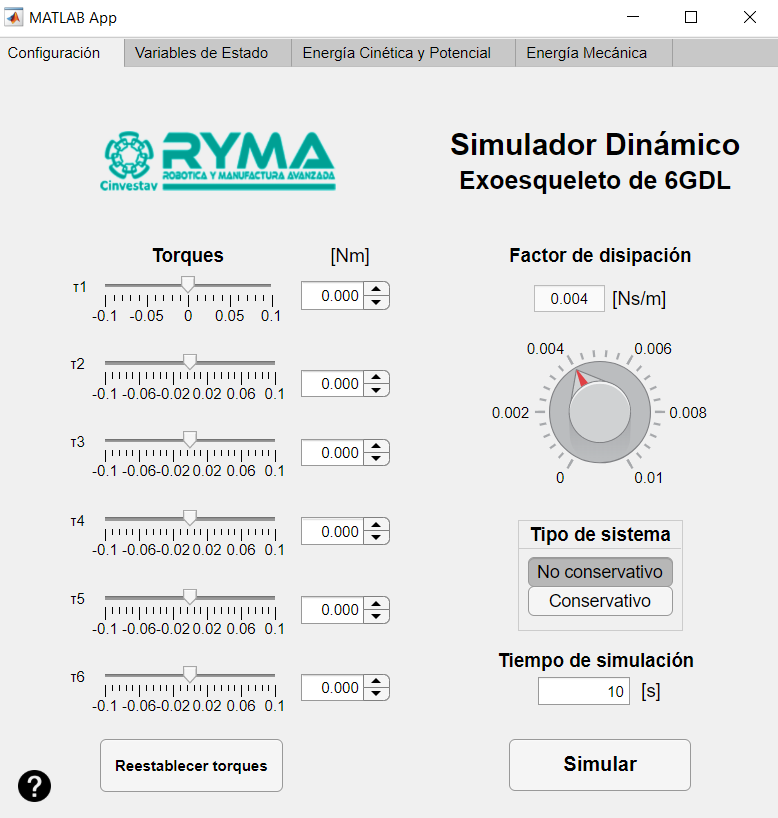
\includegraphics[scale = 0.4]{GUI.png}
        \centering
        \caption{ Interfaz Gráfica de Usuario }
        \label{fig:GUI}
    \end{figure}

\subsection{Visualizador}
    Por otra parte, se buscó complementar la interfaz gráfica con una visualización del comportamiento
    del exoesqueleto. Para ello, se optó por el uso de \emph{Simscape} \cite{simscape} y \emph{Simscape Multibody} \cite{SimscapeMultibody}, 
    permitiendo la construcción del diagrama de bloques en \emph{Simulink} de la Figura \ref{fig:visualizador}.
    Donde la única entrada son las coordenadas generalizadas $\boldsymbol{q}$.

    Para ello, se exportó el modelo 3D (Figura \ref{fig:3DModel}) previamente diseñado en \emph{SolidWorks} a un archivo
    \emph{URDF} \cite{urdf} mediante la extesión desarrollada por \cite{sw2urdf} bajo el procediento en \cite{import_urdf}. 

    Obteniendo el resultado de la Figura \ref{fig:visualizador}, donde se anuló el motor dinámico de 
    \emph{Simscape} para no modificar ningun resultado previamente obtenido por el simulador desarrollado.
    \begin{figure}[H]
        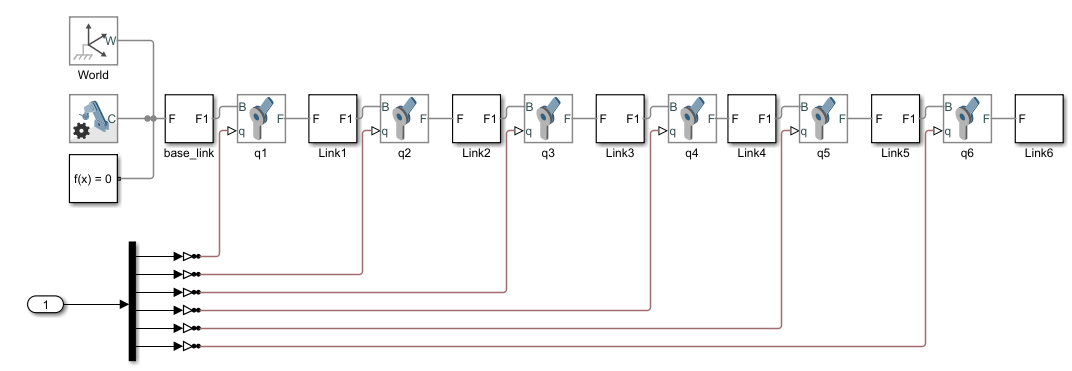
\includegraphics[scale = 0.233]{simscape.png}
        \centering
        \caption{Diagrama de bloques del visualizador}
        \label{fig:visualizador}
    \end{figure}
    Del mismo modo, al culminar la simulación se construyen las vistas de la Figura \ref{fig:vistas} que permiten observar desde diferentes
    puntos el comportamiento del exoesqueleto. 
    \begin{figure}[h]
        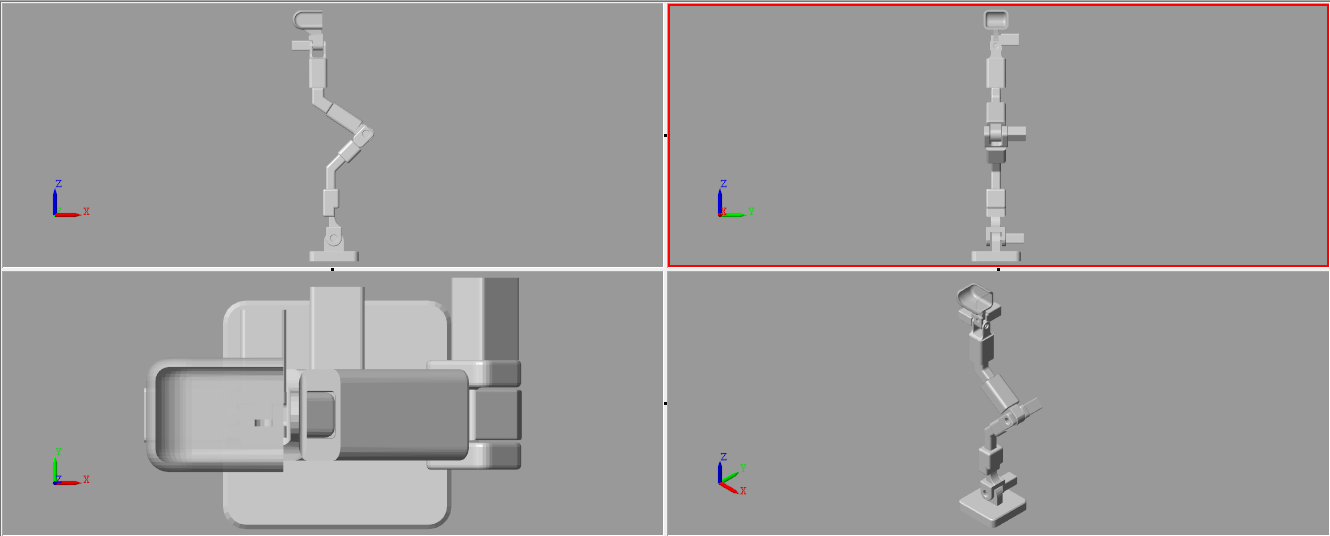
\includegraphics[scale = 0.156]{vistas_out.png}
        \centering
        \caption{ Vistas del simulador }
        \label{fig:vistas}
    \end{figure}
    
    